% !TeX program = xelatex
\documentclass[12pt,a4paper,oneside]{report}

\usepackage[a4paper,top=2.5cm,bottom=2.5cm,left=3cm,right=2.5cm]{geometry}
\usepackage{fontspec}
\usepackage[vietnamese]{babel}
\usepackage{graphicx}
\usepackage{booktabs}
\usepackage{colortbl}
\usepackage{longtable}
\usepackage{array}
\usepackage{tabularx}
\usepackage{float}
\usepackage{caption}
\usepackage{subcaption}
\usepackage{xcolor}
\usepackage{tikz}
\usepackage{eso-pic}
\usepackage{amsmath}
\usepackage{listings}
\usepackage{enumitem}
\usepackage{hyperref}
\usepackage[nameinlink,noabbrev]{cleveref}
\usepackage{fancyhdr}
\usepackage{setspace}
\usepackage{titlesec}
\usepackage{csquotes}
\DeclareQuoteAlias{english}{vietnamese}
\usepackage[backend=biber,style=ieee,sorting=none]{biblatex}

\addbibresource{references.bib}
\graphicspath{{images/}}
\definecolor{chapterblue}{RGB}{0,43,92}
\definecolor{sectionblue}{RGB}{0,91,161}
\definecolor{subsectionblue}{RGB}{35,126,190}
\definecolor{subsubsectionblue}{RGB}{74,151,205}
\definecolor{accentblue}{RGB}{0,112,192}
\definecolor{lightblue}{RGB}{232,243,252}
\definecolor{codeblue}{RGB}{243,248,252}
\colorlet{navyblue}{chapterblue}

\hypersetup{
    colorlinks=true,
    linkcolor=sectionblue,
    citecolor=sectionblue,
    urlcolor=accentblue,
    pdftitle={Báo cáo đồ án cuối kỳ Trực quan hóa dữ liệu}
}

\setmainfont{Times New Roman}
\setstretch{1.25}
\setlength{\parindent}{1.25cm}
\setlength{\parskip}{0.25em}
\setlist{nosep}
\setlist[itemize]{label=\textcolor{subsectionblue}{\textbullet}}

\titleformat{\chapter}[display]
  {\bfseries\color{chapterblue}\raggedright}
  {\Large CHƯƠNG \thechapter}
  {0.4em}
  {\LARGE}
\titleformat{\section}
  {\Large\bfseries\color{sectionblue}}
  {\thesection}
  {0.7em}
  {}
\titleformat{\subsection}
  {\large\bfseries\color{subsectionblue}}
  {\thesubsection}
  {0.7em}
  {}
\titleformat{\subsubsection}
  {\normalsize\bfseries\color{subsubsectionblue}}
  {\thesubsubsection}
  {0.7em}
  {}
\titlespacing*{\section}{0pt}{2.2ex plus 0.5ex}{0.8ex}
\titlespacing*{\subsection}{0pt}{1.8ex plus 0.4ex}{0.6ex}
\titlespacing*{\subsubsection}{0pt}{1.4ex plus 0.3ex}{0.5ex}

\captionsetup{
    labelfont={bf,color=sectionblue},
    textfont={color=chapterblue}
}
\arrayrulecolor{black}

\pagestyle{fancy}
\setlength{\headheight}{26pt}
\fancyhf{}
\fancyhead[L]{\color{black}Đồ án Trực quan hóa dữ liệu}
\fancyhead[R]{\color{black}\ProjectShortTitle}
\fancyfoot[C]{\color{chapterblue}\thepage}
\renewcommand{\headrulewidth}{0.4pt}
\renewcommand{\headrule}{\hbox to\headwidth{\color{black}\leaders\hrule height \headrulewidth\hfill}}

\lstset{
    backgroundcolor=\color{codeblue},
    basicstyle=\ttfamily\small,
    breaklines=true,
    frame=single,
    rulecolor=\color{subsectionblue},
    numbers=left,
    numberstyle=\tiny\color{subsectionblue},
    keywordstyle=\bfseries\color{sectionblue},
    commentstyle=\itshape\color{subsectionblue},
    stringstyle=\color{chapterblue},
    showstringspaces=false,
    tabsize=2
}

% ==================== THONG TIN CAN CAP NHAT ====================
\newcommand{\UniversityName}{Đại học Quốc gia Thành phố Hồ Chí Minh}
\newcommand{\SchoolName}{Trường Đại học Khoa học Tự nhiên}
\newcommand{\FacultyName}{Khoa Công nghệ Thông tin}
\newcommand{\CourseName}{Trực quan hóa dữ liệu}
\newcommand{\ProjectTitle}{Vietnam Climate Pulse: Khám phá Khí hậu và Thời tiết Cực đoan Việt Nam}
\newcommand{\ProjectShortTitle}{Vietnam Climate Pulse}
\newcommand{\TeamName}{Nhóm 1}
\newcommand{\TeamMembers}{Lê Lâm Trí Đức -- 23120237, Hoàng Quốc Việt -- 23120189, Nguyễn Lê Thế Vinh -- 23120190, Phạm Quang Vinh -- 23120202}
\newcommand{\InstructorName}{Bùi Tiến Lên}
\newcommand{\ReportDate}{tháng 06, năm 2026}
% ===============================================================

\begin{document}

\pagenumbering{gobble}
% Trang bia giu phong cach cua mau mon hoc truoc: khung vien doi, logo va tong navy.
\begin{titlepage}
\AddToShipoutPictureBG*{%
    \AtPageLowerLeft{%
        \put(\LenToUnit{1.2cm},\LenToUnit{1.2cm}){%
            \color{navyblue}\linethickness{2.5pt}%
            \framebox(
                \LenToUnit{\dimexpr\paperwidth-2.4cm\relax},
                \LenToUnit{\dimexpr\paperheight-2.4cm\relax}
            ){}%
        }%
        \put(\LenToUnit{1.45cm},\LenToUnit{1.45cm}){%
            \color{navyblue}\linethickness{0.8pt}%
            \framebox(
                \LenToUnit{\dimexpr\paperwidth-2.9cm\relax},
                \LenToUnit{\dimexpr\paperheight-2.9cm\relax}
            ){}%
        }%
    }%
}

\begin{center}
\vspace*{0.35cm}

{\fontsize{13}{15}\selectfont\bfseries\color{navyblue}
\MakeUppercase{\UniversityName}}\\[0.2cm]
{\fontsize{13}{15}\selectfont\bfseries\color{navyblue}
\MakeUppercase{\SchoolName}}\\[0.15cm]
{\fontsize{11}{13}\selectfont\bfseries\color{navyblue}
\MakeUppercase{\FacultyName}}

\vspace{0.45cm}

\includegraphics[width=4.8cm, keepaspectratio]{images/logo_khtn.png}
\vspace{0.4cm}

{\color{navyblue}\rule{0.75\textwidth}{1pt}}
\vspace{0.35cm}

{\fontsize{14}{16}\selectfont\bfseries\color{navyblue}
BÁO CÁO ĐỒ ÁN CUỐI KỲ}\\[0.25cm]
{\fontsize{12}{14}\selectfont\bfseries\color{navyblue}
Môn: \CourseName}

\vspace{0.45cm}
{\color{navyblue}\rule{0.75\textwidth}{1pt}}
\vspace{0.65cm}

{\fontsize{18}{22}\selectfont\bfseries\color{navyblue}
\MakeUppercase{\ProjectTitle}}
\end{center}

\vspace*{\fill}

\begin{flushleft}
\hspace{2.1cm}
\begin{minipage}{0.72\textwidth}
{\fontsize{12}{16}\selectfont\bfseries\color{navyblue}
Nhóm thực hiện: \TeamName}\\[0.2cm]
{\fontsize{12}{16}\selectfont\bfseries\color{navyblue}
Thành viên: \TeamMembers}\\[0.2cm]
{\fontsize{12}{16}\selectfont\bfseries\color{navyblue}
Giảng viên hướng dẫn: \InstructorName}
\end{minipage}
\end{flushleft}

\vspace{0.7cm}
\begin{center}
{\fontsize{11}{13}\selectfont\itshape\color{navyblue}
Thành phố Hồ Chí Minh, \ReportDate}
\end{center}
\vspace{0.25cm}
\end{titlepage}

\chapter*{Lời cam đoan}
\addcontentsline{toc}{chapter}{Lời cam đoan}

Nhóm cam đoan báo cáo và sản phẩm là kết quả làm việc của nhóm. Mọi nguồn dữ liệu,
tài liệu, mã nguồn và công cụ AI được sử dụng đều được công bố minh bạch và trích
dẫn phù hợp. Nhóm chịu trách nhiệm về tính chính xác của nội dung, kết quả phân tích
và các quyết định được đưa ra dựa trên hỗ trợ của AI.

\vspace{1.5cm}
\begin{flushright}
Đại diện nhóm thực hiện\\[1.5cm]
\textit{[Họ tên]}
\end{flushright}


\chapter*{Tóm tắt}
\addcontentsline{toc}{chapter}{Tóm tắt}

\textit{Viết khoảng 200--300 từ, trình bày bối cảnh Việt Nam, vấn đề cần giải quyết,
dữ liệu, phương pháp trực quan hóa, cách tích hợp AI, các kết quả nổi bật và đóng góp
chính của dự án. Không đưa thông tin chưa được chứng minh bởi dữ liệu.}

\noindent\textbf{Từ khóa:} [từ khóa 1], [từ khóa 2], trực quan hóa dữ liệu, phân tích dữ liệu, AI.


\chapter*{Phân công và Đóng góp Thành viên}
\addcontentsline{toc}{chapter}{Phân công và Đóng góp Thành viên}

Bảng phân công trách nhiệm và tỷ lệ đóng góp của các thành viên trong nhóm 1:

\begin{longtable}{|p{0.20\textwidth}|>{\centering\arraybackslash}p{0.12\textwidth}|p{0.42\textwidth}|>{\centering\arraybackslash}p{0.16\textwidth}|}
\hline
\textbf{Thành viên} & \textbf{MSSV} & \textbf{Công việc phụ trách} & \textbf{Mức độ đóng góp} \\ \hline
\endhead
Lê Lâm Trí Đức & 23120237 & Nhóm trưởng, thiết kế giao diện React, tích hợp ECharts bản đồ trạm đo và các biểu đồ xu hướng. & 100\% \\ \hline
Hoàng Quốc Việt & 23120189 & Phát triển pipeline dữ liệu Python, kết nối API Open-Meteo, xử lý lỗi rate-limit và xuất tệp Parquet sạch. & 100\% \\ \hline
Nguyễn Lê Thế Vinh & 23120190 & Xây dựng Backend FastAPI, kết nối cơ sở dữ liệu DuckDB local-first và viết các API endpoint phục vụ dashboard. & 100\% \\ \hline
Phạm Quang Vinh & 23120202 & Phát triển module AI Analyst, viết bộ kiểm soát an toàn SQL Guard, kiểm thử unit test tự động và viết báo cáo LaTeX. & 100\% \\ \hline
\end{longtable}



\pagenumbering{roman}
\tableofcontents
\listoffigures
\listoftables
\clearpage

\pagenumbering{arabic}
\chapter{Khởi nguồn và Ý nghĩa Đề tài}

\section{Bối cảnh và động lực}
Việt Nam là một trong những quốc gia chịu ảnh hưởng nặng nề nhất bởi biến đổi khí hậu toàn cầu. Sự gia tăng tần suất và cường độ của các hiện tượng thời tiết cực đoan như nắng nóng gay gắt, hạn mặn và mưa lũ dị thường đã và đang tác động trực tiếp đến đời sống dân sinh, an ninh nguồn nước và sự phát triển kinh tế bền vững. Tuy nhiên, dữ liệu khí tượng thô thường rất phức tạp, phân tán và khó tiếp cận đối với đại đa số công chúng, sinh viên hoặc các nhà hoạch định chính sách phổ thông. Động lực của đề tài này là xây dựng một hệ thống trực quan hóa trực quan, sinh động để chuyển hóa dữ liệu số thô kệch thành các tri thức khí hậu dễ hiểu, phục vụ giáo dục, truyền thông và nghiên cứu cộng đồng.

\section{Phát biểu vấn đề}
Bài toán trung tâm của nghiên cứu được xác định là đánh giá diễn biến khí hậu và nhận diện các hiện tượng thời tiết cực đoan tại Việt Nam giai đoạn 2020-2025. Để làm rõ và giải quyết triệt để bài toán này, nhóm nghiên cứu tập trung khai thác ba khía cạnh phân tích cốt lõi liên quan chặt chẽ đến sự biến động thời tiết cục bộ.

Khía cạnh thứ nhất tập trung vào việc mô tả đặc trưng khí hậu ba miền nhằm trực quan hóa sự phân hóa sâu sắc về nhiệt độ trung bình, biên độ nhiệt và lượng mưa tích lũy giữa miền Bắc mang tính chất cận nhiệt đới biên độ rộng, miền Trung chịu tác động khắc nghiệt của gió phơn Tây Nam, và miền Nam với đặc thù nhiệt đới gió mùa ổn định quanh năm. Khía cạnh thứ hai hướng đến xây dựng thuật toán tự động nhận diện và thống kê các giá trị cực đoan, từ đó phát hiện, định lượng và lập bản đồ phân bố các ngày xảy ra thiên tai nắng nóng gay gắt hoặc mưa lớn lịch sử tại từng địa phương. Khía cạnh thứ ba nghiên cứu mối quan hệ tương quan đa biến giữa các thông số vật lý như bức xạ mặt trời, nhiệt độ, lượng mưa và tốc độ gió nhằm đúc kết những quy luật vật lý và xu hướng tác động mang tính khoa học.

\section{Mục tiêu nghiên cứu}
Mục tiêu tổng quát của nghiên cứu này là thiết lập một ứng dụng trực quan hóa tương tác (dashboard) về khí hậu Việt Nam theo kiến trúc cục bộ nhằm tối ưu hóa hiệu năng, đồng thời tích hợp trợ lý trí tuệ nhân tạo hỗ trợ phân tích ngôn ngữ tự nhiên.

Về mặt trực quan hóa và khai phá dữ liệu, nghiên cứu hướng tới việc bản đồ hóa 28 trạm quan trắc khí tượng trọng điểm trên toàn lãnh thổ, đồng thời xây dựng các biểu đồ phân tích xu hướng thời gian theo chu kỳ tháng và biểu đồ nhiệt độ năm dưới dạng ma trận nhiệt độ. Hệ thống cũng tích hợp chức năng lọc động và thống kê các sự kiện cực đoan dựa trên các tham số ngưỡng linh hoạt do người dùng tùy chọn, kết hợp tính toán trực tiếp hệ số tương quan Pearson đa biến nhằm phục vụ nghiên cứu liên hệ vật lý. Song song với đó, mục tiêu tích hợp mô hình ngôn ngữ lớn làm trợ lý ảo nhằm mục đích hỗ trợ người dùng phi kỹ thuật dễ dàng tạo và thực thi các câu lệnh truy vấn SQL từ ngôn ngữ tự nhiên một cách an toàn và có kiểm soát thông qua cơ chế phê duyệt thủ công.

\section{Câu hỏi phân tích}
Để cụ thể hóa các mục tiêu trên, nghiên cứu đặt ra bốn nhóm câu hỏi phân tích thời tiết cốt lõi trong thực tế:
\begin{enumerate}
    \item \textbf{Về mặt tổng quan địa lý:} Miền nào có nền nhiệt độ trung bình cao nhất cả nước và sự khác biệt nhiệt độ nền giữa ba miền Bắc, Trung, Nam biến động ra sao trong giai đoạn sáu năm khảo sát?
    \item \textbf{Về xu hướng thời gian:} Chu kỳ mùa mưa của miền Trung dịch chuyển lệch pha như thế nào so với hai miền còn lại và liệu có dấu hiệu nóng lên toàn cầu thông qua sự gia tăng nhiệt độ nền hàng năm hay không?
    \item \textbf{Đối với phân tích mối quan hệ vật lý:} Mối tương quan thuận nghịch giữa bức xạ mặt trời sóng ngắn và nhiệt độ không khí trung bình ngày thể hiện thế nào, và lượng mưa lớn cùng độ phủ mây tác động ra sao tới lượng bức xạ nhận được?
    \item \textbf{Về mặt cực đoan khí hậu:} Những địa phương nào có tần suất nắng nóng gay gắt lớn nhất, và thời điểm cũng như lượng mưa của đợt thiên tai mưa lớn lịch sử tại khu vực miền Trung là bao nhiêu để hỗ trợ đưa ra các khuyến cáo an toàn?
\end{enumerate}
\newpage
\section{Đối tượng sử dụng và phạm vi nghiên cứu}
Đối tượng sử dụng hướng tới của ứng dụng bao gồm học sinh, sinh viên học tập trong các khối ngành địa lý và khoa học môi trường cần số liệu trực quan thực nghiệm, các tuyên truyền viên về biến đổi khí hậu cần công cụ trực quan hóa sinh động, và cộng đồng dân cư quan tâm đến các chỉ số thời tiết địa phương.

Về phạm vi không gian, nghiên cứu giới hạn phân tích tại 28 trạm quan trắc khí tượng phân bố đều trên khắp lãnh thổ Việt Nam, đại diện cho các đặc thù vi khí hậu lục địa và hải đảo. Về phạm vi thời gian, dữ liệu được khai thác liên tục trong giai đoạn sáu năm, từ ngày 01 tháng 01 năm 2020 đến hết ngày 31 tháng 12 năm 2025. Cần lưu ý rằng hệ thống được thiết kế hoàn toàn cho mục đích phân tích, mô tả trực quan dữ liệu khí hậu lịch sử và không tích hợp các mô hình dự báo thời tiết ngắn hạn hoặc trung hạn trong tương lai.

\section{Đóng góp chính}
Đóng góp chính của nghiên cứu này nằm ở việc phát triển một giải pháp trực quan hóa khí hậu Việt Nam toàn diện, kết hợp chặt chẽ giữa kỹ thuật xử lý dữ liệu và công nghệ giao diện tương tác. Nghiên cứu đã xây dựng một bộ dữ liệu khí hậu lịch sử đồng bộ, sạch và đáng tin cậy bao gồm hơn 61.000 bản ghi của 28 trạm đo. Đồng thời, nhóm phát triển một dashboard tương tác cao cấp sử dụng thư viện kết xuất đồ họa ECharts để hiển thị bản đồ phân bố trạm đo địa lý và các xu hướng tương quan đa biến. Cuối cùng, việc tích hợp module trợ lý AI hoạt động minh bạch dưới cơ chế giám sát thủ công đảm bảo khả năng truy xuất dữ liệu hiệu năng cao và an toàn bảo mật tuyệt đối trên nền tảng DuckDB cục bộ.

\chapter{Dữ liệu}

\section{Nguồn dữ liệu và độ tin cậy}
\begin{longtable}{p{0.18\textwidth}p{0.26\textwidth}p{0.16\textwidth}p{0.28\textwidth}}
\toprule
\textbf{Nguồn} & \textbf{Đơn vị cung cấp/URL} & \textbf{Ngày truy cập} & \textbf{Lý do tin cậy và giấy phép} \\
\midrule
\textit{Nguồn 1} & \textit{Đơn vị và liên kết} & \textit{Ngày} & \textit{Mô tả} \\
\textit{Nguồn 2} & \textit{Đơn vị và liên kết} & \textit{Ngày} & \textit{Mô tả} \\
\bottomrule
\end{longtable}

\section{Mô tả bộ dữ liệu}
Nêu đơn vị quan sát, số dòng, số cột, phạm vi thời gian, phạm vi địa lý và định dạng.
Xác nhận bộ dữ liệu có tối thiểu 2.000 dòng và 7 biến độc lập.

\section{Data dictionary}
Trình bày các biến quan trọng tại \cref{app:data-dictionary}; phân biệt biến gốc,
biến dẫn xuất, biến định lượng và định tính.

\section{Thu thập và tái tạo dữ liệu}
Mô tả cách tải dữ liệu, tham số, phiên bản, cấu trúc thư mục và lệnh chạy pipeline.
Nêu cách bảo đảm người khác có thể tái tạo bộ dữ liệu phân tích.

\section{Làm sạch và biến đổi}
\begin{itemize}
    \item Chuẩn hóa kiểu dữ liệu, tên biến, đơn vị và địa danh Việt Nam.
    \item Xử lý giá trị thiếu, ngoại lệ và bản ghi trùng lặp.
    \item Kết hợp các nguồn và tạo biến dẫn xuất.
    \item Bảo toàn dữ liệu gốc và lưu dấu vết xử lý.
\end{itemize}

\section{Đánh giá chất lượng dữ liệu}
Trình bày tỷ lệ thiếu, trùng lặp, ngoại lệ, kiểm tra miền giá trị và các giới hạn.
Giải thích tác động của chất lượng dữ liệu lên kết luận.

\section{Đạo đức, quyền riêng tư và hạn chế}
Nêu giấy phép, quyền riêng tư, thiên lệch dữ liệu và các trường hợp không nên diễn
giải quá mức.

\chapter{Phương pháp và Quy trình Kỹ thuật}

\section{Quy trình phân tích và Luồng dữ liệu}
Quy trình phân tích dữ liệu trong dự án được triển khai qua các bước tuần tự từ đầu đến cuối. Khởi đầu bằng việc thu thập dữ liệu, hệ thống tự động hóa quá trình truy vấn thông tin khí hậu lịch sử từ dịch vụ API dựa trên danh sách các trạm đo đại diện tại Việt Nam. Tiếp theo, quá trình tiền xử lý và làm sạch sẽ chuyển đổi dữ liệu khí quyển thô thành cấu trúc bảng phẳng chuẩn hóa, bổ sung thông tin vùng miền địa lý, và tối ưu hóa định dạng lưu trữ nhằm tiết kiệm bộ nhớ. Đối với việc truy vấn dữ liệu, hệ thống thiết lập một cơ chế truy xuất cục bộ hiệu năng cao để đọc trực tiếp dữ liệu đã làm sạch mà không cần qua các hệ quản trị trung gian cồng kềnh. Backend chịu trách nhiệm tiếp nhận, định tuyến và tính toán các số liệu thống kê tổng hợp để cung cấp dữ liệu qua các điểm kết nối dịch vụ cho Frontend. Cuối cùng, ở bước trực quan hóa tương tác, ứng dụng phía máy khách tiếp nhận dữ liệu để kết xuất các biểu đồ và bản đồ địa lý sinh động, đồng thời quản lý luồng phê duyệt các truy vấn nâng cao từ module trợ lý trí tuệ nhân tạo.

\section{Phương pháp phân tích}
Dự án áp dụng ba phương pháp phân tích dữ liệu chính để khai phá tri thức khí hậu Việt Nam. Phương pháp thứ nhất là thống kê mô tả và gom nhóm, sử dụng các hàm tổng hợp như tính giá trị trung bình, tối đa, tối thiểu và tổng của DuckDB để tính toán nhiệt độ trung bình, lượng mưa năm và biên độ nhiệt của từng trạm đo hoặc gom nhóm theo vùng miền và tháng trong năm nhằm tìm kiếm quy luật mùa vụ. Phương pháp thứ hai là lọc ngưỡng cực đoan nhằm tự động phát hiện các ngày thời tiết dị thường thông qua bộ lọc động dựa trên phép so sánh lớn hơn hoặc bằng các giá trị ngưỡng tùy chỉnh của nhiệt độ và lượng mưa. Phương pháp thứ ba là phân tích tương quan đa biến, thực hiện tính toán trực tiếp hệ số tương quan Pearson giữa các cặp biến số đo lường liên tục bằng hàm tương quan tích hợp của DuckDB để xác định mối liên hệ vật lý giữa nhiệt độ, lượng mưa, sức gió và bức xạ mặt trời.

\section{Thiết kế trực quan và Mã hóa thị giác}
Để tối ưu hóa trải nghiệm phân tích của người dùng, nhóm nghiên cứu đã chọn lọc kỹ lưỡng các kỹ thuật mã hóa thị giác tương thích với đặc thù dữ liệu. Đầu tiên, bản đồ phân bố trạm đo được xây dựng dưới dạng biểu đồ phân tán Scatter Plot bằng cách sử dụng vĩ độ làm trục tung và kinh độ làm trục hoành, phác họa hình dáng tự nhiên của lãnh thổ Việt Nam, trong đó kích thước điểm được mã hóa theo nhiệt độ trung bình và màu sắc phân biệt theo vùng miền. Tiếp theo, biểu đồ đường chuỗi thời gian dạng đường trơn được lựa chọn để thể hiện xu hướng nhiệt độ tối đa, tối thiểu và trung bình theo tháng, giúp trực quan hóa biên độ nhiệt và biến động theo mùa. Đối với lượng mưa, do đặc trưng tích lũy của chỉ số này, biểu đồ cột Bar Chart là phương án tối ưu để so sánh tổng lượng mưa giữa các tháng. Cuối cùng, ma trận Heatmap Tháng x Năm mã hóa nhiệt độ trung bình bằng các ô màu chuyển sắc từ xanh lạnh sang đỏ đậm, giúp phát hiện tức thì các chu kỳ mùa vụ và sự bất thường thời tiết qua các năm.

\section{Storytelling và cấu trúc thông tin}
Cấu trúc thông tin của ứng dụng tuân thủ triết lý thiết kế thông tin nổi tiếng của Ben Shneiderman là xem tổng quan trước, lọc và phóng to, và hiển thị chi tiết khi có nhu cầu. Tại cấp độ thứ nhất về tổng quan quốc gia, người dùng được tiếp cận bản đồ phân bố toàn bộ các trạm đo và các chỉ số trung bình của cả nước. Cấp độ thứ hai cho phép lọc địa phương khi người dùng chọn một trạm đo cụ thể trên bản đồ để cập nhật bảng số liệu chi tiết của địa phương đó hoặc lọc theo trạm tại phân hệ khám phá xu hướng. Cấp độ thứ ba hướng tới khai thác tương quan nâng cao và tích hợp trí tuệ nhân tạo, cho phép người dùng chuyển sang phòng thí nghiệm tương quan hoặc tương tác trực tiếp với trợ lý AI để thực thi các truy vấn SQL sâu trên toàn bộ cơ sở dữ liệu.

\section{Kiến trúc hệ thống và Công nghệ lựa chọn}
Hệ thống được thiết kế theo kiến trúc xử lý cục bộ (local-first) tinh gọn và bảo mật cao thông qua bốn tầng chức năng chính. Tầng lưu trữ sử dụng định dạng nén cột nhằm tối ưu dung lượng đĩa và tốc độ đọc/ghi dữ liệu. Tầng dịch vụ backend chịu trách nhiệm tính toán và thực thi các câu lệnh truy vấn dữ liệu trực tiếp trên tệp lưu trữ mà không cần triển khai hệ quản trị cơ sở dữ liệu máy chủ độc lập phức tạp. Tầng hỗ trợ trí tuệ nhân tạo tích hợp bộ dịch ngôn ngữ tự nhiên thành mã lệnh truy vấn dữ liệu, được trang bị module kiểm soát an toàn nghiêm ngặt để phát hiện và ngăn chặn các nguy cơ phá hủy dữ liệu, đồng thời tự động lưu lại nhật ký lịch sử tương tác. Cuối cùng, tầng giao diện frontend vận hành như một ứng dụng đơn trang tương tác cao, đảm nhận vai trò hiển thị trực quan các biểu đồ động và tiếp nhận các phản hồi điều khiển của người dùng.


\chapter{Thiết kế Giao diện và Trải nghiệm Tương tác}

\section{Tổng quan giao diện}
Dashboard ứng dụng được thiết kế trên một giao diện thống nhất theo phong cách Dark Mode hiện đại, sử dụng các thẻ khối bán trong suốt (glassmorphism) giúp tăng chiều sâu thị giác và tạo cảm giác premium. Thanh sidebar bên trái cố định dùng để điều hướng giữa năm phân hệ chức năng chính bao gồm Tổng quan trạm đo phục vụ hiển thị bản đồ toàn quốc và chỉ số chi tiết trạm, Khám phá khí hậu thể hiện xu hướng nhiệt độ và ma trận nhiệt độ mùa vụ, Thời tiết cực đoan cung cấp thống kê ngày vượt ngưỡng thiên tai, Tương quan khí hậu biểu diễn hệ số Pearson đa biến, và cuối cùng là phân hệ AI Analyst Portal hỗ trợ phân tích ngôn ngữ tự nhiên.

\begin{figure}[H]
    \centering
    \fbox{\parbox[c][7cm][c]{0.85\textwidth}{\centering
    \textbf{KHOẢNG TRỐNG CHÈN ẢNH GIAO DIỆN TỔNG QUAN DASHBOARD}\\
    \textit{Hướng dẫn đặt tên tệp:} \texttt{dashboard\_overview.png}\\
    \textit{Đường dẫn lưu tệp trên đĩa:} \texttt{report/images/dashboard\_overview.png}\\
    \textit{Mô tả:} Chụp ảnh giao diện chính lúc đang hiển thị tab Tổng quan, có đầy đủ bản đồ trạm đo và các thẻ KPI phía trên.}}
    \caption{Giao diện tổng quan của dashboard Vietnam Climate Pulse}
    \label{fig:dashboard-overview}
\end{figure}

\section{Các biểu đồ chính và chức năng}
Mỗi phân hệ giao diện tập trung giải quyết các bài toán trực quan hóa chuyên sâu:

\subsection{Phân hệ Khám phá Khí hậu (Explorer)}
Trang này được thiết kế để phân tích các yếu tố chu kỳ và xu hướng thời gian của từng địa phương:
\begin{figure}[H]
    \centering
    \fbox{\parbox[c][5cm][c]{0.85\textwidth}{\centering
    \textbf{KHOẢNG TRỐNG CHÈN ẢNH PHÂN HỆ KHÁM PHÁ KHÍ HẬU}\\
    \textit{Hướng dẫn đặt tên tệp:} \texttt{dashboard\_explorer.png}\\
    \textit{Đường dẫn lưu tệp trên đĩa:} \texttt{report/images/dashboard\_explorer.png}\\
    \textit{Mô tả:} Chụp ảnh giao diện tab Khám phá khí hậu, thể hiện biểu đồ đường nhiệt độ tối đa/trung bình/tối thiểu và biểu đồ heatmap tháng x năm.}}
    \caption{Giao diện phân hệ khám phá khí hậu và xu hướng mùa vụ}
    \label{fig:dashboard-explorer}
\end{figure}

\subsection{Phân hệ Thời tiết Cực đoan (Extreme Events)}
Trang này hỗ trợ lọc động và khoanh vùng các địa điểm thường xuyên xuất hiện các đợt nắng nóng hoặc mưa bão lịch sử:
\begin{figure}[H]
    \centering
    \fbox{\parbox[c][5cm][c]{0.85\textwidth}{\centering
    \textbf{KHOẢNG TRỐNG CHÈN ẢNH PHÂN HỆ THỜI TIẾT CỰC ĐOAN}\\
    \textit{Hướng dẫn đặt tên tệp:} \texttt{dashboard\_extreme.png}\\
    \textit{Đường dẫn lưu tệp trên đĩa:} \texttt{report/images/dashboard\_extreme.png}\\
    \textit{Mô tả:} Chụp ảnh giao diện tab Thời tiết cực đoan, bao gồm hai thanh trượt điều chỉnh ngưỡng nhiệt độ/lượng mưa và bảng nhật ký các ngày cực đoan bên dưới.}}
    \caption{Giao diện phân hệ thống kê và hiển thị nhật ký thời tiết cực đoan}
    \label{fig:dashboard-extreme}
\end{figure}

\section{Liên kết tương tác giữa các biểu đồ}
Ứng dụng thiết lập cơ chế liên kết tương tác chặt chẽ giữa các thành phần trực quan nhằm tối ưu hóa khả năng khám phá thông tin. Cụ thể, hệ thống tích hợp tính năng click chọn trên bản đồ địa lý, theo đó khi người dùng nhấp chuột vào một chấm tròn đại diện cho trạm đo trên bản đồ, hệ thống sẽ tự động bắt sự kiện và cập nhật tức thì dữ liệu của bảng thông tin chi tiết địa phương thông qua đồng bộ trạng thái trong React. Thêm vào đó, tính năng đồng bộ tooltip theo trục chung được cấu hình cho các biểu đồ đường và cột trong phân hệ khám phá, hỗ trợ hiển thị đồng thời thông số của nhiều biến số khi người dùng rê chuột, tạo điều kiện thuận lợi cho việc đối chiếu nhanh giá trị tại cùng một thời điểm.

\section{Bộ lọc và điều hướng}
Để nâng cao tính cá nhân hóa trong việc khai thác dữ liệu, hệ thống cung cấp các bộ lọc và điều hướng tương tác động. Bộ chọn dropdown tại phân hệ Khám phá khí hậu cho phép người dùng lọc thông tin chi tiết của từng trạm đo cụ thể hoặc xem số liệu trung bình trên quy mô toàn quốc, tự động cập nhật đồng bộ các biểu đồ đường, biểu đồ cột và ma trận nhiệt độ tương ứng. Hơn nữa, các thanh trượt động được tích hợp trong bộ lọc ngưỡng thời tiết cực đoan, cho phép người dùng kéo trượt để thay đổi giá trị ngưỡng nhiệt độ hoặc lượng mưa, hệ thống sẽ tự động gửi tham số mới về API backend và tải lại danh sách các ngày thiên tai tương ứng.

\section{Thiết kế thẩm mỹ và khả năng tiếp cận}
Tính thẩm mỹ và khả năng tiếp cận của ứng dụng được chú trọng thiết kế nhằm mang lại trải nghiệm tối ưu cho nhiều đối tượng người dùng. Bảng màu của dashboard sử dụng các gam màu có ý nghĩa chỉ thị khí hậu trực quan, trong đó màu đỏ (\texttt{\#ff5b52}) tượng trưng cho nắng nóng cực đoan, màu xanh ngọc (\texttt{\#00bcd4}) đại diện cho mưa bão tích lũy, và màu xanh dương (\texttt{\#00d2ff}) phản ánh nền nhiệt độ thấp lạnh giá. Đồng thời, thiết kế đáp ứng (Responsive) được triển khai thông qua CSS Grid và Media Queries, tự động ẩn thanh điều hướng sidebar và chuyển đổi bố cục từ hai cột thành một cột dọc trên màn hình thiết bị di động và máy tính bảng, đảm bảo tính thân thiện và tối ưu hiển thị trên mọi loại thiết bị.


\chapter{Khám phá Tri thức và Phân tích Thực nghiệm}

\section{Bức tranh tổng quan}
Thông qua việc phân tích và trực quan hóa bộ dữ liệu hơn 61.000 dòng ghi nhận trong giai đoạn 2020-2025 tại 28 trạm quan trắc, dự án đã mô hình hóa thành công bức tranh khí hậu tổng thể của Việt Nam. Kết quả thống kê chỉ ra nhiệt độ trung bình toàn quốc dao động quanh mức $25.1^\circ$C. Lượng mưa trung bình năm của các địa phương đạt khoảng 1.500 mm đến 2.500 mm. Các trạm đo phân bố dọc theo chiều dài đất nước đã phản ánh rõ nét sự phân hóa khí hậu đa dạng theo cả vĩ độ và địa hình vùng miền. Phần phân tích chi tiết bên dưới được tổ chức bám sát theo ba phân hệ biểu đồ chính của dashboard (\Cref{fig:dashboard-explorer,fig:dashboard-extreme,fig:dashboard-relationship}), mỗi phân hệ gồm bốn biểu đồ tương ứng.

\section{Phân hệ Khám phá Khí hậu (Explorer)}
Phân hệ này gồm bốn biểu đồ được hiển thị đồng thời trên bố cục lưới $2\times2$ (\Cref{fig:dashboard-explorer}), phục vụ phân tích chu kỳ mùa vụ và xu hướng dài hạn của từng địa phương hoặc toàn quốc.

\subsection{Chu kỳ nhiệt độ theo tháng}
Biểu đồ đường (\Cref{fig:explorer-tempcycle}) thể hiện ba đường nhiệt độ tối đa, trung bình và tối thiểu theo từng tháng trong năm. Kết quả cho thấy tính mùa vụ nhiệt độ rõ rệt trên cả nước, với biên độ dao động giữa tháng nóng nhất và tháng lạnh nhất đặc biệt lớn ở miền Bắc do ảnh hưởng của gió mùa Đông Bắc, trong khi miền Nam gần như duy trì nền nhiệt ổn định quanh năm.

\subsection{Lượng mưa trung bình theo tháng}
Biểu đồ cột (\Cref{fig:explorer-rain}) thể hiện lượng mưa trung bình tích lũy theo từng tháng. Phân tích chu kỳ thời gian theo tháng đã làm nổi bật sự dịch chuyển lượng mưa rõ rệt giữa các vùng miền. Tại miền Bắc, mùa mưa chủ yếu kéo dài từ tháng 6 đến tháng 9, trùng khớp với thời kỳ mùa hè nóng ẩm, trong khi mùa đông từ tháng 12 đến tháng 2 năm sau ghi nhận nền lượng mưa rất thấp kèm theo nhiệt độ giảm sâu. Trái lại, miền Trung thể hiện một sự dịch chuyển mùa mưa rõ rệt về phía cuối năm, với lượng mưa tích lũy đạt đỉnh điểm vào các tháng 10 và tháng 11 -- kết quả tác động tổ hợp của địa hình dãy Trường Sơn chắn gió mùa Đông Bắc mang hơi ẩm và sự đổ bộ tập trung của các cơn bão nhiệt đới trong giai đoạn này. Đối với miền Nam, khí hậu phân hóa thành hai mùa mưa và khô rõ rệt, trong đó mùa mưa kéo dài từ tháng 5 đến tháng 11 dưới ảnh hưởng của gió mùa Tây Nam nóng ẩm, giúp lượng mưa trung bình tháng luôn duy trì ở ngưỡng cao.

\subsection{Xu hướng nhiệt độ trung bình theo năm}
Biểu đồ đường có tô nền (\Cref{fig:explorer-yearly}) tổng hợp nhiệt độ trung bình toàn quốc theo từng năm trong giai đoạn 2020-2025, cho phép quan sát nhanh xu hướng biến động nhiệt độ liên năm mà không bị nhiễu bởi dao động mùa vụ ngắn hạn trong từng tháng.

\subsection{Heatmap mùa vụ nhiệt độ (Tháng × Năm)}
Ma trận nhiệt (heatmap, \Cref{fig:explorer-heatmap}) với trục hoành là tháng, trục tung là năm và màu sắc biểu diễn nhiệt độ trung bình ngày, cho phép đối chiếu đồng thời tính chu kỳ mùa vụ (theo hàng) và xu hướng liên năm (theo cột) trên cùng một biểu đồ. Cách trình bày này giúp phát hiện trực quan các ô có màu đậm bất thường, tương ứng với các tháng nóng cực đoan như tháng 4 năm 2024.

\section{Phân hệ Thời tiết Cực đoan (Extreme Events)}
Phân hệ này cho phép người dùng điều chỉnh ngưỡng nắng nóng và ngưỡng mưa lớn bằng thanh trượt động, đồng thời lọc theo địa điểm; bốn biểu đồ trong \Cref{fig:dashboard-extreme} tự động cập nhật theo tham số ngưỡng được chọn.

\subsection{So sánh ngày cực đoan giữa các trạm}
Biểu đồ cột nhóm (\Cref{fig:extreme-compare}) xếp hạng Top 10 trạm đo có số ngày vượt ngưỡng nắng nóng và mưa lớn nhiều nhất, hỗ trợ thao tác nhấp chuột để khoanh vùng (drill-down) vào một trạm cụ thể. Nghiên cứu đã phát hiện đợt nắng nóng diện rộng cực kỳ khốc liệt vào cuối tháng 4 năm 2024: trạm khí tượng Lào Cai ở miền Bắc ghi nhận giá trị nhiệt độ kỷ lục \textbf{$41.8^\circ$C} vào ngày \textbf{29/04/2024}, đồng thời trạm Huế ở miền Trung cũng ghi nhận mức nhiệt cực đại \textbf{$41.5^\circ$C} vào ngày \textbf{30/04/2024}.

\subsection{Bản đồ điểm nóng thời tiết cực đoan}
Bản đồ địa lý Việt Nam (\Cref{fig:extreme-map}) hiển thị vị trí 28 trạm đo dưới dạng các điểm có kích thước tỷ lệ thuận với tổng số ngày cực đoan (nắng nóng cộng mưa lớn) ghi nhận được, giúp nhận diện nhanh các khu vực chịu ảnh hưởng thời tiết cực đoan nặng nề nhất trên bản đồ thay vì phải đọc bảng số liệu. Về các hiện tượng mưa cực đoan trong ngày, trạm Vinh ở miền Trung ghi nhận lượng mưa tích lũy kỷ lục trong ngày lên tới \textbf{267.5 mm} vào ngày \textbf{18/10/2020}, dẫn tới ngập lụt nghiêm trọng trên diện rộng, trong khi trạm Rạch Giá ở miền Nam ghi nhận lượng mưa cực đại trong ngày đạt mức \textbf{261.5 mm} vào ngày \textbf{05/10/2021}.

\subsection{Xu hướng ngày cực đoan theo năm}
Biểu đồ đường hai chuỗi (\Cref{fig:extreme-yearly}) (nắng nóng và mưa lớn) theo từng năm cho phép quan sát liệu tần suất các hiện tượng cực đoan có xu hướng gia tăng qua thời gian hay không, phục vụ trực tiếp cho việc minh họa tác động của biến đổi khí hậu bằng số liệu thực nghiệm thay vì nhận định định tính.

\subsection{Phân bố ngày cực đoan theo tháng}
Biểu đồ cột nhóm (\Cref{fig:extreme-monthly}) thể hiện tính mùa vụ của thời tiết cực đoan, cho thấy các ngày nắng nóng tập trung chủ yếu vào giai đoạn tháng 4 đến tháng 6, trong khi các ngày mưa lớn tập trung vào giai đoạn tháng 9 đến tháng 11 -- trùng khớp với cao điểm mùa bão tại Việt Nam.

\section{Phân hệ Tương quan Khí hậu (Relationship Lab)}
Phân hệ này khai thác các mối quan hệ thống kê đa biến trên toàn bộ 61.376 quan sát, không có bộ lọc động, tập trung vào bốn góc nhìn tương quan bổ trợ lẫn nhau (\Cref{fig:dashboard-relationship}).

\subsection{Ma trận tương quan Pearson}
Ma trận nhiệt $4\times4$ (\Cref{fig:relationship-corr}) tính hệ số tương quan Pearson giữa bốn biến: nhiệt độ trung bình, lượng mưa, tốc độ gió và bức xạ mặt trời. Hệ số tương quan giữa bức xạ mặt trời sóng ngắn tích lũy ngày (\texttt{shortwave\_radiation\_sum}) và nhiệt độ không khí trung bình ngày (\texttt{temperature\_2m\_mean}) đạt mức \textbf{0.5606}, thể hiện mối tương quan thuận từ mức trung bình đến mạnh -- lượng bức xạ mặt trời cao thúc đẩy quá trình hấp thụ nhiệt lượng của bề mặt đất, từ đó gián tiếp làm tăng nhiệt độ không khí ở tầng sát đất. Bên cạnh đó, lượng mưa ngày ghi nhận mối tương quan nghịch với bức xạ mặt trời, đạt giá trị khoảng $-0.25$ tại các vùng thuộc miền Nam, phản ánh quy luật thời tiết thực tế khi những ngày có lượng mưa lớn thường đi kèm độ phủ mây dày, cản trở đáng kể lượng bức xạ sóng ngắn chiếu trực tiếp xuống bề mặt đất.

\subsection{Bức xạ mặt trời và nhiệt độ trung bình theo miền}
Biểu đồ phân tán (\Cref{fig:relationship-radiation}) đối chiếu bức xạ mặt trời với nhiệt độ trung bình ngày, tô màu theo ba miền Bắc -- Trung -- Nam để phát hiện sự khác biệt về độ nhạy tương quan giữa các vùng khí hậu. Kết quả cho thấy hệ số tương quan đạt giá trị mạnh nhất tại miền Bắc \textbf{(0.6022)}, mức trung bình tại miền Nam \textbf{(0.5681)} và yếu nhất tại miền Trung \textbf{(0.4796)}. Điều này chỉ ra nhiệt độ không khí tại miền Trung chịu sự chi phối mạnh mẽ bởi các yếu tố động lực học khí quyển phức tạp, chẳng hạn như hiệu ứng phơn vượt dãy Trường Sơn, chứ không đơn thuần phụ thuộc vào lượng bức xạ mặt trời nhận được tại chỗ như hai miền còn lại.

\subsection{Vĩ độ và nhiệt độ trung bình}
Biểu đồ phân tán thứ hai (\Cref{fig:relationship-latitude}) đối chiếu vĩ độ địa lý của từng trạm đo với nhiệt độ trung bình ngày, trực quan hóa trực tiếp quy luật "càng ra Bắc càng lạnh" của khí hậu Việt Nam. Phân tích thực nghiệm chứng minh miền Nam có nền nhiệt độ trung bình ngày ổn định và cao nhất cả nước ($27.16^\circ$C) với biên độ nhiệt cực nhỏ, thể hiện qua độ lệch chuẩn chỉ $1.32^\circ$C. Ngược lại, miền Bắc sở hữu nhiệt độ trung bình thấp nhất ($23.32^\circ$C) nhưng có biên độ dao động nhiệt rộng nhất cả nước với độ lệch chuẩn lên tới $4.91^\circ$C. Trong khi đó, miền Trung có nền nhiệt độ trung bình nằm ở khoảng trung gian ($24.80^\circ$C).

\subsection{Phân bố nhiệt độ theo miền}
Biểu đồ hộp (box plot, \Cref{fig:relationship-boxplot}) kết hợp lớp điểm ngoại lai tổng hợp toàn bộ phân bố nhiệt độ trung bình ngày theo từng miền, bổ trợ trực quan cho hai biểu đồ phân tán ở trên bằng cách thể hiện rõ khoảng tứ phân vị, trung vị và các giá trị bất thường. Dải nhiệt độ miền Nam dao động trong khoảng hẹp từ $22.3^\circ$C đến $33.6^\circ$C, trong khi miền Bắc ghi nhận nhiệt độ cực tiểu giảm sâu xuống $4.5^\circ$C vào mùa đông và nhiệt độ cực đại đạt $33.9^\circ$C vào mùa hè -- thể hiện qua các điểm ngoại lai kéo dài ở hai đầu hộp. Miền Trung lại ghi nhận giá trị nhiệt độ tối đa ngày cao nhất lên tới $35.3^\circ$C do ảnh hưởng trực tiếp của gió phơn Tây Nam khô nóng, xuất hiện dưới dạng điểm ngoại lai phía trên hộp.

\section{Hàm ý và giới hạn diễn giải}
Về mặt ứng dụng thực tiễn, kết quả trực quan hóa này hỗ trợ các chuyên gia truyền thông môi trường truyền tải hiệu quả thông điệp về tính khốc liệt của biến đổi khí hậu thông qua các đợt nắng nóng lịch sử năm 2024. Đồng thời, công cụ này giúp sinh viên ngành khí tượng thủy văn dễ dàng đối chiếu lý thuyết về tương quan đa biến và tính chu kỳ mùa bằng các số liệu thực nghiệm sinh động. Tuy nhiên, về mặt giới hạn diễn giải, dữ liệu tái phân tích của Open-Meteo có thể có những sai lệch nhỏ so với số liệu quan trắc thực tế bằng nhiệt kế cơ học của Việt Nam trong một số hiện tượng vi khí hậu cục bộ như sương muối hay mưa đá. Do đó, người dùng không nên sử dụng bộ dữ liệu này cho các ứng dụng kỹ thuật có yêu cầu độ chính xác tuyệt đối hoặc lập kế hoạch dự báo nông nghiệp ngắn hạn.

\chapter{Tích hợp Trí tuệ Nhân tạo và An toàn Hệ thống}

\section{Mục tiêu và phạm vi AI}
Module AI trong dự án đóng vai trò là một trợ lý phân tích dữ liệu chuyên sâu (AI Analyst), hỗ trợ người dùng khám phá các mối liên hệ hoặc trích xuất số liệu từ tệp dữ liệu khí hậu nằm ngoài các tính năng tĩnh của dashboard. Về mặt công nghệ, hệ thống sử dụng mô hình ngôn ngữ lớn Google Gemini (\texttt{gemini-flash-latest}) truy cập qua API, kèm cơ chế dự phòng chạy ngoại tuyến (mock offline) khi không cấu hình khóa API nhằm bảo đảm quá trình trình diễn và chấm điểm cục bộ luôn hoạt động ngay cả khi mất kết nối. Tác vụ AI được giới hạn ở việc sinh mã truy vấn chỉ đọc -- dưới dạng câu lệnh SQL trên DuckDB hoặc đoạn mã Python/pandas tùy người dùng lựa chọn -- kèm giải thích ý nghĩa, và tuyệt đối không được phép can thiệp vào mã nguồn backend hoặc chỉnh sửa dữ liệu gốc.

\section{Nguyên tắc không thực thi ngầm}
Dự án tuân thủ nghiêm ngặt nguyên tắc minh bạch dữ liệu và duy trì sự kiểm soát của con người (Human-in-the-loop) đối với mọi hoạt động của hệ thống. Theo đó, mô hình trí tuệ nhân tạo không bao giờ được phép tự động hoặc âm thầm thực thi bất kỳ truy vấn SQL nào trực tiếp vào cơ sở dữ liệu. Mọi mã nguồn SQL do AI khởi tạo đều bắt buộc phải hiển thị một cách tường minh và trực quan trên giao diện người dùng ở trạng thái chờ duyệt. Hơn nữa, người dùng hoàn toàn có quyền can thiệp, chỉnh sửa cấu trúc hoặc nội dung cú pháp SQL này ngay trong trình biên soạn văn bản trước khi đưa ra quyết định thực thi. Hệ thống chỉ chính thức chạy truy vấn trên nền DuckDB sau khi nhận được lệnh xác nhận phê duyệt một cách chủ động từ phía người dùng qua hành động nhấn nút kích hoạt trên giao diện.

\section{Luồng phê duyệt của người dùng}
Quy trình thực thi truy vấn an toàn được thiết kế thông qua các bước phối hợp chặt chẽ giữa frontend và backend. Ban đầu, người dùng nhập câu hỏi bằng ngôn ngữ tự nhiên tại giao diện trợ lý AI, chẳng hạn như yêu cầu so sánh nền nhiệt độ cực đại giữa Sa Pa và Đà Lạt. Sau đó, giao diện gửi yêu cầu này tới API backend, truyền kèm ngữ cảnh cấu trúc bảng dữ liệu để dịch thành mã SQL thô. Khi nhận được kết quả dịch kèm giải thích logic từ AI Service, frontend sẽ hiển thị đề xuất này dưới dạng bản nháp tạm thời (DRAFT). Tại đây, người dùng tiến hành rà soát cấu trúc cú pháp câu lệnh, thực hiện các hiệu chỉnh cần thiết và quyết định nhấn nút duyệt chạy. Lúc này, hệ thống kích hoạt module kiểm soát an toàn để xác thực tính hợp lệ của câu lệnh, nếu vượt qua kiểm tra, DuckDB sẽ thực thi trực tiếp trên tệp Parquet cục bộ và trả kết quả dạng bảng hiển thị lên màn hình. Cuối cùng, toàn bộ quá trình tương tác sẽ được tự động ghi nhận vào cơ sở dữ liệu nhật ký kiểm toán.

\section{Thiết kế API}
Trách nhiệm giữa các API được phân định rõ ràng nhằm đảm bảo tính bảo mật và độc lập:
\begin{table}[htbp]
\centering
\renewcommand{\arraystretch}{1.25}
\begin{tabularx}{\textwidth}{|p{0.35\textwidth}|X|}
\hline
\textbf{API Endpoint} & \textbf{Trách nhiệm chi tiết} \\ \hline
\texttt{POST /api/ai/}\newline\texttt{proposals} & Tiếp nhận câu hỏi kèm ngữ cảnh lược đồ dữ liệu, gọi Gemini dịch thành mã nháp (SQL hoặc Python) và lời giải thích. Chưa thực thi. Trạng thái lưu: \texttt{draft}. \\ \hline
\texttt{POST /api/ai/}\newline\texttt{proposals/\{id\}/}\newline\texttt{approve} & Tiếp nhận mã SQL người dùng gửi lên sau khi duyệt/chỉnh sửa. Chạy bộ kiểm tra an toàn và lưu trạng thái \texttt{approved}. \\ \hline
\texttt{POST /api/ai/}\newline\texttt{proposals/\{id\}/}\newline\texttt{execute} & Chỉ cho phép chạy nếu đề xuất có trạng thái \texttt{approved}. Kết nối DuckDB thực thi SQL cục bộ, trả kết quả và lưu trạng thái \texttt{executed}. \\ \hline
\end{tabularx}
\caption{Phân tách trách nhiệm giữa các API AI}
\end{table}

\section{Hiển thị code và giải thích trên giao diện}
Giao diện người dùng được thiết kế để hiển thị đồng thời mã SQL đề xuất trong một khung biên soạn mã và một khung văn bản giải thích logic truy vấn:

\begin{figure}[htbp]
    \centering
    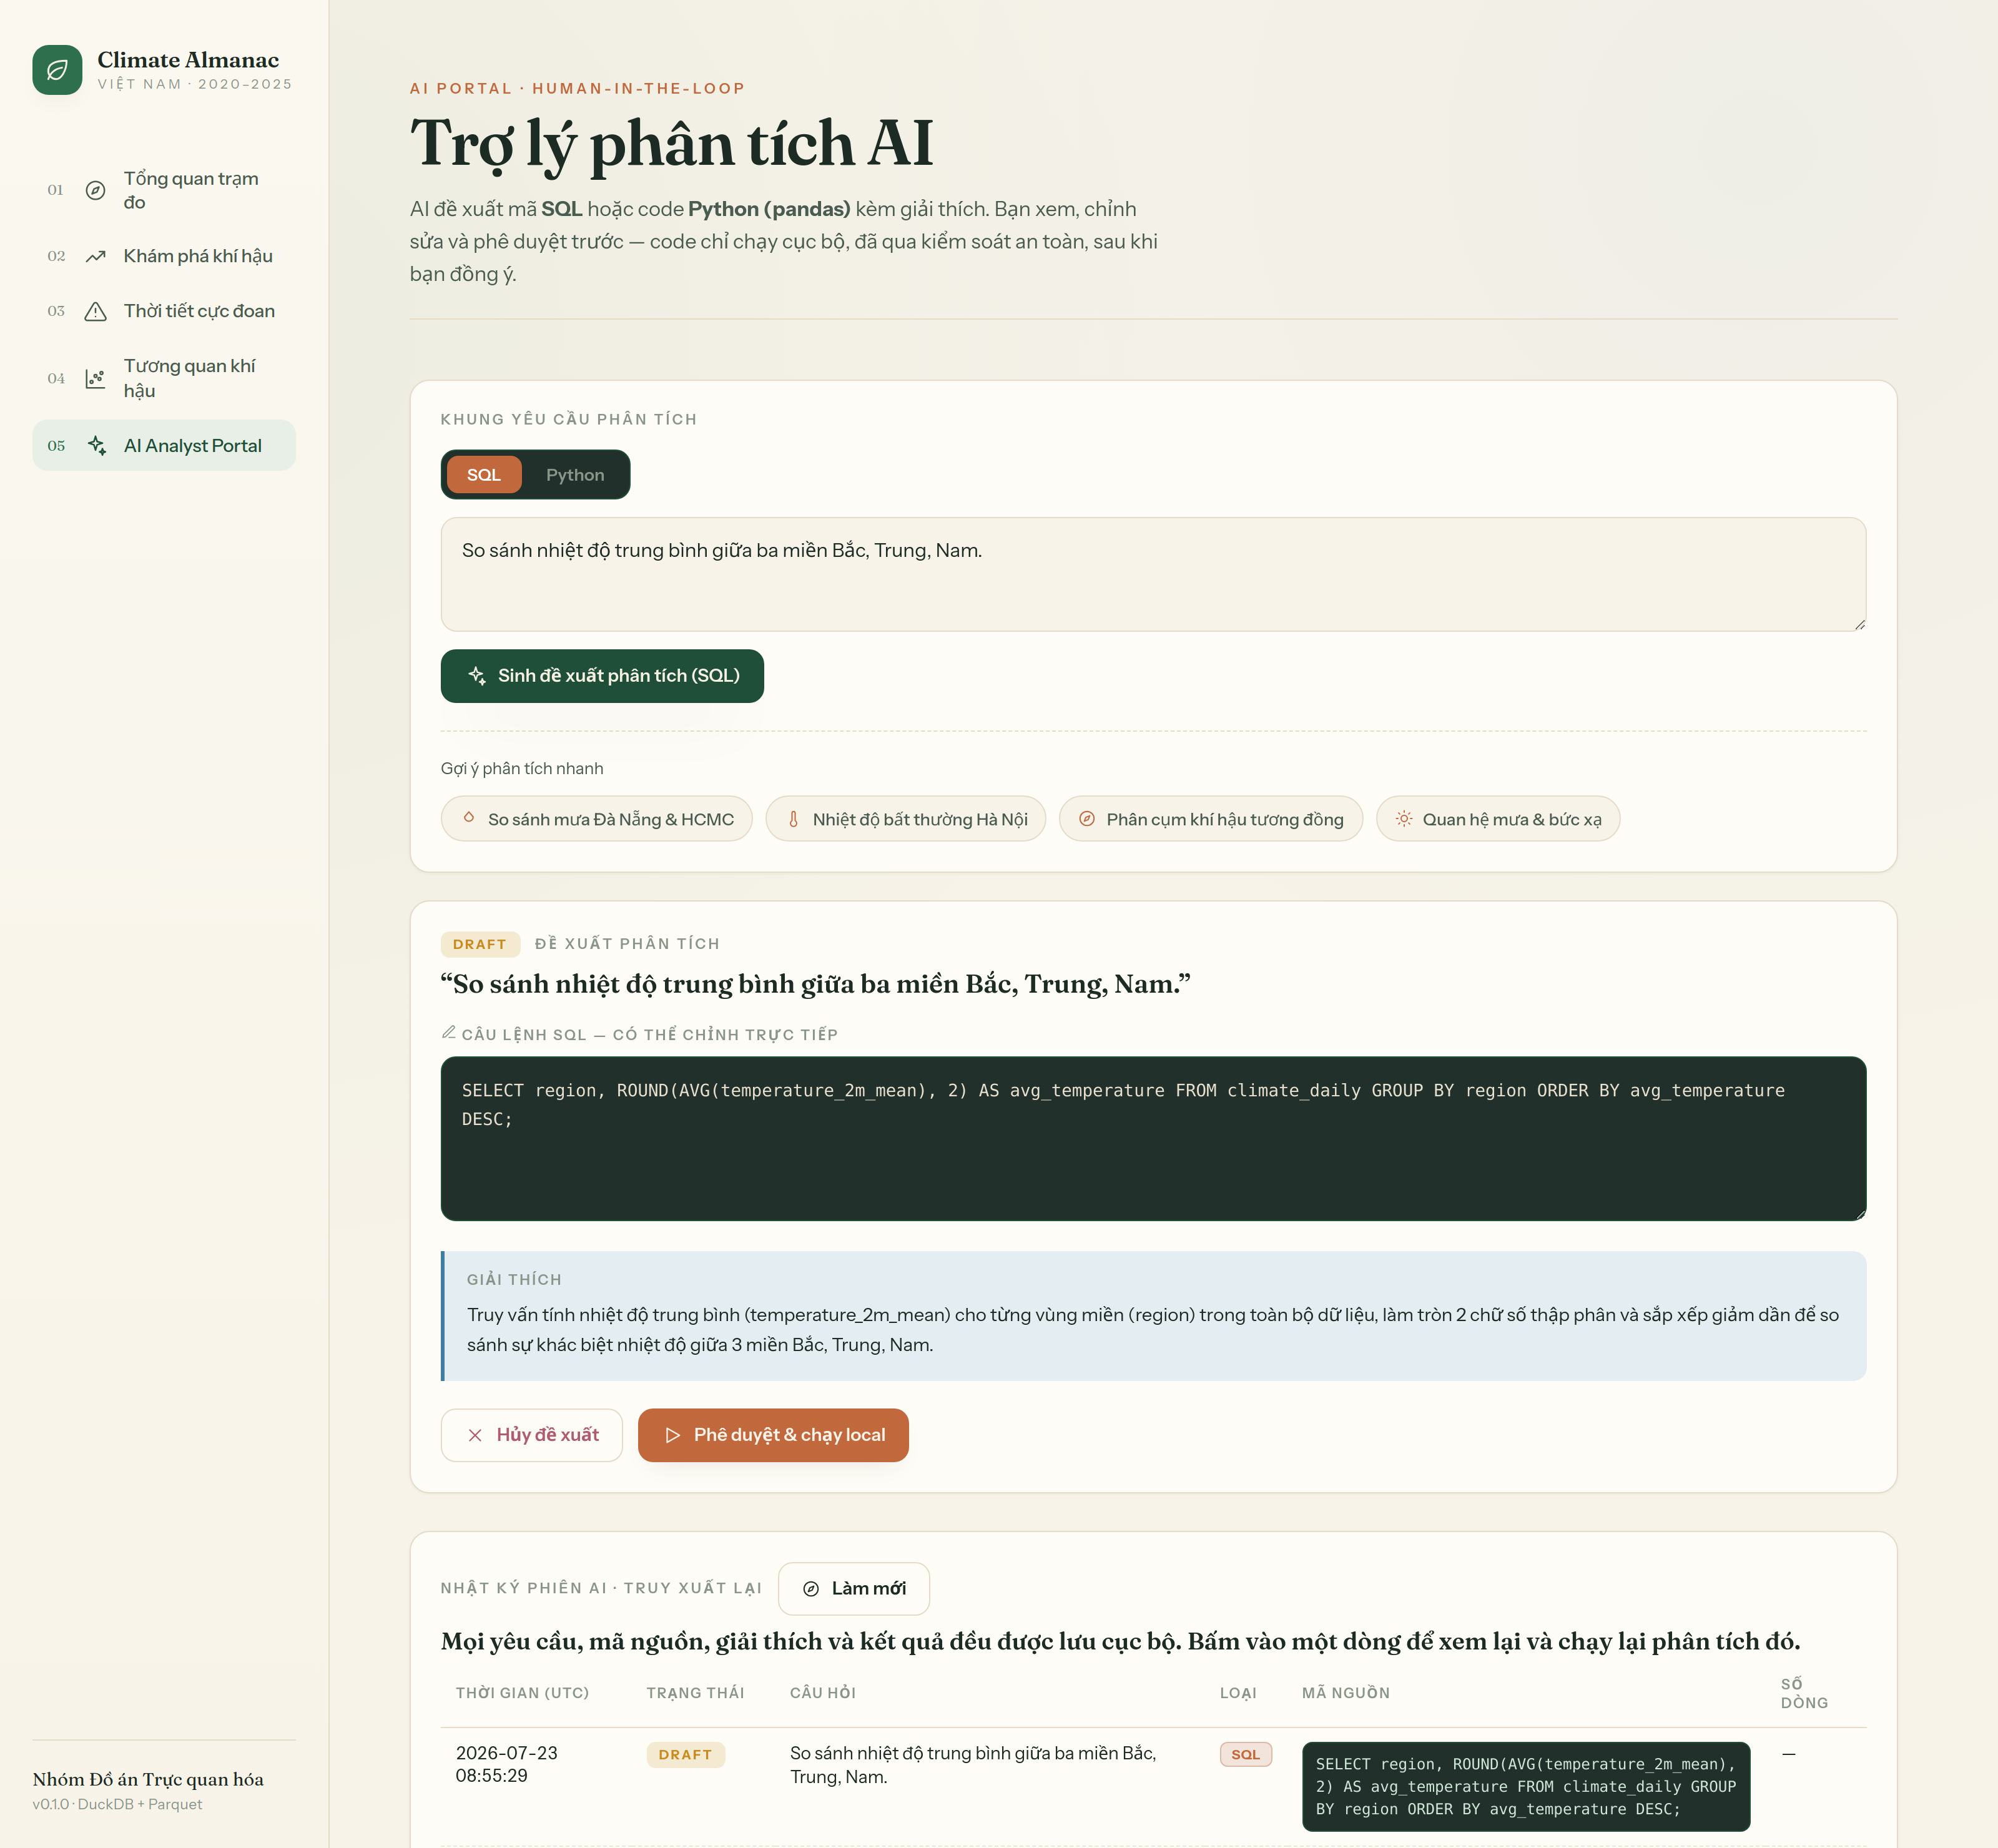
\includegraphics[width=0.82\textwidth]{dashboard_ai_analyst.png}
    \caption{Giao diện quản lý đề xuất và phê duyệt thực thi câu lệnh SQL của AI}
    \label{fig:dashboard-ai-analyst}
\end{figure}

\section{Kiểm soát an toàn truy vấn (Guardrails)}
Để bảo vệ an toàn cho cơ sở dữ liệu cục bộ, hệ thống được trang bị bộ lọc an toàn chuyên biệt để thực hiện xác thực nghiêm ngặt mã lệnh SQL trước khi chuyển giao cho động cơ truy vấn. Quy trình kiểm soát này được xây dựng trên ba lớp phòng ngự chính. Đầu tiên là cơ chế kiểm tra đặc quyền chỉ đọc, sử dụng thuật toán phân tích cú pháp để bắt buộc mọi câu lệnh gửi lên phải bắt đầu bằng các từ khóa truy xuất dữ liệu an toàn. Lớp phòng ngự thứ hai là danh sách cấm, ngăn chặn triệt để các câu lệnh có khả năng làm thay đổi tính toàn vẹn của dữ liệu hoặc phá hủy cấu trúc bảng. Cuối cùng, hệ thống thực hiện cơ chế chặn đa lệnh bằng cách chỉ cho phép thực thi duy nhất một truy vấn đơn lẻ trong mỗi phiên tương tác, loại trừ hoàn toàn nguy cơ chèn nhiều câu lệnh liên tiếp phân tách bằng ký tự đặc biệt. Đối với chế độ phân tích bằng Python/pandas, một bộ kiểm soát riêng phân tích cây cú pháp trừu tượng (AST) của đoạn mã để chặn triệt để mọi lệnh \texttt{import}, các hàm nguy hiểm như \texttt{eval}, \texttt{exec}, \texttt{open} cùng việc truy cập các thuộc tính đặc biệt (\enquote{dunder}); nhờ đó đoạn mã chỉ được phép tính toán thuần túy trên khung dữ liệu đã nạp sẵn mà không thể đọc/ghi tệp hay gọi mạng.

\section{Lưu trữ và khả năng kiểm toán (Audit Log)}
Toàn bộ nhật ký hoạt động của trợ lý trí tuệ nhân tạo được tự động ghi nhận vào cơ sở dữ liệu nhật ký kiểm toán chuyên dụng của hệ thống. Cơ chế ghi nhật ký được thiết kế để lưu giữ toàn diện các thông tin phục vụ mục đích giám sát hoạt động. Các thuộc tính lưu trữ bao gồm khóa định danh phiên tương tác duy nhất, nhãn thời gian thực thi, và nội dung câu hỏi ban đầu của người dùng. Ngoài ra, hệ thống cũng lưu trữ song song mã truy vấn do AI đề xuất ban đầu và mã truy vấn thực tế được người dùng phê duyệt chạy, cùng với trạng thái kết quả thực thi và thông tin chi tiết lỗi hệ thống trong trường hợp truy vấn gặp sự cố. Điều này đảm bảo tính minh bạch và cho phép quản trị viên dễ dàng rà soát hành vi của AI.

\section{Đánh giá chất lượng và Quá trình sử dụng}
Quá trình đánh giá thực nghiệm thông qua tập câu hỏi kiểm thử đa dạng cho thấy trợ lý AI hoạt động ổn định và chính xác. Các tác vụ phức tạp như so sánh lượng mưa giữa các khu vực địa lý, lọc nhiệt độ bất thường cục bộ hay tính toán hệ số tương quan đa biến đều được mô hình chuyển đổi thành mã SQL tối ưu cho DuckDB với thời gian xử lý cực ngắn. Hơn nữa, việc duy trì vai trò chủ động của con người giúp đảm bảo tính linh hoạt tối đa cho hệ thống. Trong trường hợp mô hình sinh ra câu lệnh có tên cột chưa khớp hoàn toàn hoặc bộ lọc chưa thực sự tối ưu, người dùng có thể chủ động sửa đổi trực tiếp trên giao diện để hoàn thiện câu lệnh trước khi thực thi, tạo nên cơ chế cộng tác hiệu quả giữa người dùng và trí tuệ nhân tạo.


\chapter{Đánh giá và kiểm thử}

\section{Đối chiếu yêu cầu đề bài}
\begin{longtable}{p{0.38\textwidth}p{0.15\textwidth}p{0.35\textwidth}}
\toprule
\textbf{Yêu cầu} & \textbf{Trạng thái} & \textbf{Bằng chứng} \\
\midrule
Dữ liệu Việt Nam, tối thiểu 7 biến độc lập và 2.000 dòng & \textit{Đạt/Chưa} & \textit{Mục/hình/log} \\
Nguồn đáng tin cậy và xử lý minh bạch & \textit{Đạt/Chưa} & \textit{Mục/hình/log} \\
Biểu đồ phù hợp, rõ ràng, liên kết và tương tác & \textit{Đạt/Chưa} & \textit{Mục/hình/log} \\
Phân tích xu hướng, quan hệ biến và insight chuyên môn & \textit{Đạt/Chưa} & \textit{Mục/hình/log} \\
AI hiển thị code, giải thích và chờ phê duyệt & \textit{Đạt/Chưa} & \textit{Mục/hình/log} \\
Thực thi local và lưu đầy đủ logs & \textit{Đạt/Chưa} & \textit{Mục/hình/log} \\
\bottomrule
\end{longtable}

\section{Kiểm thử chức năng}
Liệt kê ca kiểm thử dashboard, bộ lọc, API dữ liệu, API AI, chỉnh sửa/phê duyệt,
thực thi local, logs và xử lý lỗi.

\section{Kiểm thử an toàn AI}
Trình bày kết quả khi AI sinh code sai, truy vấn ghi dữ liệu, yêu cầu ngoài phạm vi,
code chạy quá lâu hoặc người dùng từ chối phê duyệt.

\section{Đánh giá khả dụng}
Mô tả đối tượng thử nghiệm, nhiệm vụ, phản hồi, vấn đề phát hiện và thay đổi đã thực
hiện. Nếu chưa có nghiên cứu người dùng chính thức, nêu rõ giới hạn.

\section{Hiệu năng và độ ổn định}
Trình bày thời gian tải dashboard, thời gian truy vấn, thời gian phản hồi AI và hành
vi khi API/mạng không khả dụng.

\chapter{Nhật ký tương tác AI tiêu biểu}
\label{app:ai-logs}

Dưới đây là hai phiên nhật ký tiêu biểu trích xuất từ cơ sở dữ liệu nhật ký của hệ thống:

\subsection*{Phiên 1: So sánh lượng mưa miền}
\begin{table}[htbp]
\centering
\renewcommand{\arraystretch}{1.25}
\begin{tabularx}{\textwidth}{|>{\bfseries}p{0.22\textwidth}|X|}
\hline
\textbf{Trường} & \textbf{Nội dung} \\ \hline
Yêu cầu người dùng
    & So sánh lượng mưa giữa Đà Nẵng và Thành phố Hồ Chí Minh theo mùa. \\ \hline
Ngữ cảnh dữ liệu
    & Bảng dữ liệu khí hậu với các trường thông tin: ngày tháng, vị trí địa lý, lượng mưa ngày, v.v. \\ \hline
Code AI đề xuất
    & \texttt{SELECT location, month(date) as thang,} \newline
      \texttt{~~AVG(precipitation\_sum) as luong\_mua\_trung\_binh} \newline
      \texttt{FROM climate\_daily} \newline
      \texttt{WHERE location IN ('Da Nang', 'Ho Chi Minh City')} \newline
      \texttt{GROUP BY location, thang} \newline
      \texttt{ORDER BY thang, location} \\ \hline
Giải thích của AI
    & Truy vấn này tính lượng mưa trung bình theo từng tháng trong năm cho hai thành phố Đà Nẵng và TP. Hồ Chí Minh để so sánh đặc trưng mùa mưa. \\ \hline
Thay đổi của con người
    & Không thay đổi (mã đề xuất hoàn hảo). \\ \hline
Quyết định
    & Phê duyệt thực thi cục bộ. \\ \hline
Kết quả thực thi & Trả về 24 dòng dữ liệu thể hiện lượng mưa trung bình từng tháng cho 2 thành phố. \\ \hline
Nhận xét & Truy vấn chính xác, giải quyết trọn vẹn yêu cầu, tốc độ thực thi dưới 4ms. \\ \hline
\end{tabularx}
\end{table}

\subsection*{Phiên 2: Lọc nhiệt độ bất thường tại Hà Nội}
\begin{table}[htbp]
\centering
\renewcommand{\arraystretch}{1.25}
\begin{tabularx}{\textwidth}{|>{\bfseries}p{0.22\textwidth}|X|}
\hline
\textbf{Trường} & \textbf{Nội dung} \\ \hline
Yêu cầu người dùng
    & Tìm các tháng có nhiệt độ bất thường tại Hà Nội. \\ \hline
Ngữ cảnh dữ liệu
    & Bảng dữ liệu khí hậu với các trường thông tin: ngày tháng, vị trí địa lý, nhiệt độ tối đa, nhiệt độ tối thiểu. \\ \hline
Code AI đề xuất
    & \texttt{SELECT year(date) as nam, month(date) as thang,} \newline
      \texttt{~~AVG(temperature\_2m\_max) as temp\_max\_avg} \newline
      \texttt{FROM climate\_daily} \newline
      \texttt{WHERE location = 'Ha Noi'} \newline
      \texttt{GROUP BY nam, thang} \newline
      \texttt{HAVING temp\_max\_avg > 38.0} \newline
      \texttt{ORDER BY nam, thang} \\ \hline
Giải thích của AI
    & Truy vấn tính nhiệt độ trung bình tối đa theo từng tháng và lọc ra những tháng bất thường có nhiệt độ trung bình ngày nóng vượt quá 38 độ C. \\ \hline
Thay đổi của con người
    & Người dùng sửa điều kiện lọc thành \texttt{temperature\_2m\_max > 38.0} trực tiếp trong từng ngày thay vì dùng \texttt{HAVING} trên nhiệt độ trung bình tháng để tìm các ngày cực đoan thực sự. \\ \hline
Quyết định
    & Chỉnh sửa và Phê duyệt thực thi. \\ \hline
Kết quả thực thi & Trả về danh sách các ngày nắng nóng đỉnh điểm vượt ngưỡng 38°C tại Hà Nội. \\ \hline
Nhận xét & AI hỗ trợ khung mã lệnh rất tốt, người dùng đóng vai trò hiệu chỉnh điều kiện lọc chi tiết (Human-in-the-loop) để cho ra kết quả chính xác theo ý muốn. \\ \hline
\end{tabularx}
\end{table}

\chapter{Tổng kết và Hướng phát triển Tương lai}

\section{Kết quả đạt được}
Đồ án đã thiết lập thành công ứng dụng \textbf{Vietnam Climate Pulse}, giải quyết trọn vẹn bài toán trực quan hóa khí hậu Việt Nam giai đoạn 2020-2025 thông qua ba kết quả then chốt. Về mặt dữ liệu, dự án đã tự động hóa thành công quy trình thu thập dữ liệu từ dịch vụ API thời tiết, tiến hành làm sạch và lưu trữ cục bộ dưới định dạng tối ưu để tăng tốc độ truy xuất thông tin. Về trực quan hóa, nhóm đã thiết kế giao diện dashboard theo phong cách ``Editorial Climate Almanac'' tông sáng, nền giấy ấm với hệ màu đất trang nhã, biểu diễn bản đồ địa lý các trạm đo bằng biểu đồ tương tác, kết hợp biểu đồ ma trận phân tích nhiệt độ theo mùa vụ và các biểu đồ tương quan đa biến trực quan sinh động. Về tích hợp trí tuệ nhân tạo, module trợ lý phân tích đã được triển khai thành công, hỗ trợ dịch ngôn ngữ tự nhiên sang câu lệnh truy xuất dữ liệu chỉ đọc để chạy trực tiếp trên hệ thống cục bộ dưới sự kiểm soát và phê duyệt an toàn của con người.

\section{Hạn chế của đồ án}
Mặc dù đạt được đầy đủ các mục tiêu đề ra của môn học trực quan hóa dữ liệu, đồ án vẫn tồn tại một số hạn chế nhất định cần được hoàn thiện. Trước hết, do nguồn dữ liệu thời tiết lịch sử là dạng dữ liệu mô phỏng lưới toàn cầu, hệ thống có thể xuất hiện độ lệch nhỏ so với số liệu thực tế đo đạc trực tiếp bằng nhiệt kế chuyên dụng tại các trạm khí tượng quốc gia của Việt Nam. Thêm vào đó, ứng dụng hiện tại tập trung hoạt động trên môi trường máy tính cá nhân phục vụ mục đích trình diễn và kiểm thử nhanh, do đó chưa tích hợp hệ quản trị cơ sở dữ liệu máy chủ đám mây để phục vụ cho lượng người dùng lớn truy cập đồng thời trong thực tế.

\section{Hướng phát triển tương lai}
Để phát triển đồ án thành một sản phẩm nghiên cứu thực tiễn sâu rộng hơn hoặc ứng dụng thương mại, nhóm đề xuất ba hướng cải tiến trọng tâm. Hướng đi thứ nhất là tích hợp dữ liệu trạm đo thực tế bằng cách liên kết trực tiếp với hệ thống dữ liệu trực tuyến của cơ quan khí tượng thủy văn quốc gia hoặc các trạm đo tự động tại địa phương nhằm bảo đảm độ tin cậy tuyệt đối của số liệu thời gian thực. Hướng đi thứ hai tập trung mở rộng khả năng của mô hình trí tuệ nhân tạo, nâng cấp trợ lý ảo từ dịch ngôn ngữ tự nhiên sang hỗ trợ tự động thiết kế biểu đồ trực quan hoặc kết xuất báo cáo tóm tắt tri thức bằng văn bản tiếng Việt. Hướng đi cuối cùng là triển khai ứng dụng lên môi trường máy chủ đám mây trực tuyến, thiết kế lại lớp cơ sở dữ liệu phân tán kết hợp với các động cơ truy vấn chạy trực tiếp trên trình duyệt để phục vụ rộng rãi cho công chúng.


\nocite{*}
\printbibliography[heading=bibintoc,title={Tài liệu tham khảo}]

\end{document}
